\documentclass{beamer}


\usetheme{Warsaw}
\usecolortheme{crane}


\title{Partial Differentiation} 
\subtitle{Mathematical Methods in the Physical Sciences}
\author{Steve Mazza}
\institute[Naval Postgraduate School]
{ 
    Naval Postgraduate School \\
    Monterey, CA \\
    
\includegraphics[height=3cm]{images/NPS_logo.jpg}
}
\date {SE3030, Winter/2014 \\ Quantitative Methods of Systems Engineering}
\subject{Quantitative Methods of Systems Engineering}


\begin{document}

\frame{\titlepage}


\frame {{Lorenz Attractor}
	\begin{center}
		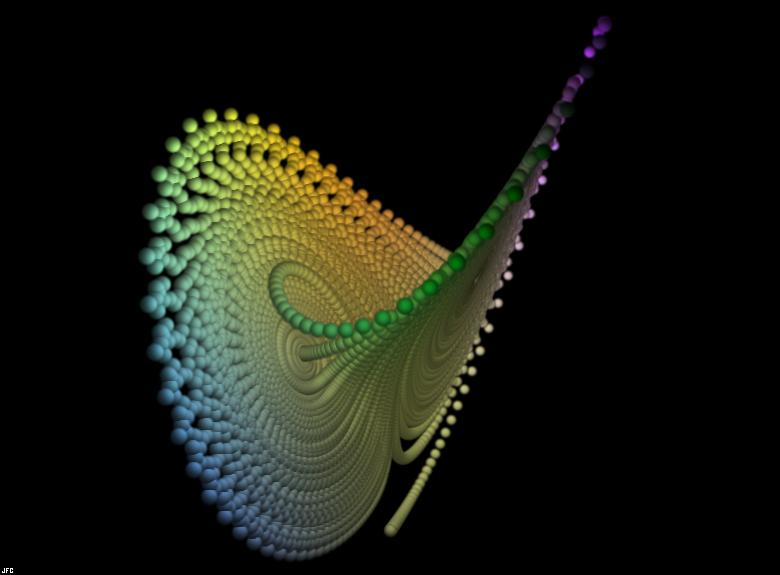
\includegraphics[width=0.8\textwidth]{images/LorenzBeads.jpg}
	\end{center}
}


\frame{{Introduction}
	\begin{block}{Definition}
		Derivatives of a multi-variable function where all variables are held fixed during differentiation except the variable of interest.
	\end{block}
	To denote this we generically write $\dfrac{\partial}{\partial r}$, which means the partial derivative with respect to $r$.  We more frequently see $\dfrac{\partial z}{\partial r}$, which means the partial derivative of $z$ with respect to $r$.  In equations of more than two variables we may see $\left(\dfrac{\partial z}{\partial r}\right)_{x}$, which denotes the partial derivative of $z$ with respect to $r$, holding $x$ constant.
}


\frame{{Example}
	\begin{exampleblock}{4.1.12}
		\begin{align*}
			z &= x^{2}+2y^{2}, x=r\text{cos}\theta, y=r\text{sin}\theta \\
	    z &= x^{2}+2y^{2} \\
	    z &= r^{2}\text{cos}^{2}\theta+2r^{2}\text{sin}^{2}\theta \\
	    \left(\dfrac{\partial z}{\partial y}\right)_{\theta}  &= r^{2}\text{cos}^{2}\theta+2r^{2}\text{sin}^{2}\theta
		\end{align*}
	\end{exampleblock}
}


\frame{{Power Series in Two Variables}
	Our standard power series expansions can be re-written as partial differential equations.
	\begin{block}{Definition}
		\[
			f(x,y) = \sum_{n=0}^{\infty}\dfrac{1}{n!}\left(h\dfrac{\partial}{\partial x}+k\dfrac{\partial}{\partial y}\right)^{n}f(a,b)
		\]
	\end{block}
	%TODO: work an example.
}


\frame{{Total Differentials}
	\begin{block}{Total Differentiation in 2 Variables}
		\[
			dz = \dfrac{\partial}{\partial x}dx+\dfrac{\partial}{\partial y}dy
		\]
	\end{block}
	\textbf{Approximation:}   For sufficiently small values of $\Delta x$ and $\Delta y$,
	\begin{itemize}
		\item $\Delta z = \Delta f = f_x(x,y)\Delta x + f_y(x,y)\Delta u$, and
		\item $f(x+\Delta x, y+\Delta y)\equiv f(x,y)+f_x(x,y)\Delta x+f_y(x,y)\Delta y$.
	\end{itemize}
}


\frame{{Approximations Using Differentials}
	\begin{exampleblock}{Example 4, Boas, p. 197}
		The relative error in length measurement is $\pm$5\% and the relative error in radius measurement is $\pm$10\%.  We want to find the largest value that $\lvert dR/R\rvert$ can have.
		\begin{align*}
			R &= \dfrac{kl}{r^2} \\
			\text{ln} R &= \text{ln} k + \text{ln} l - 2\text{ln} r \\
			\dfrac{dR}{R} &= \left\lvert\dfrac{dl}{l}\right\rvert - 2\left\lvert\dfrac{dr}{r}\right\rvert \\
			&= 0.05 + 2(0.10) \\
			&= 0.25
		\end{align*}
	\end{exampleblock}

}


\frame{{Chain Rule}
%	\begin{block}{Definition}
%		\[
%			dz = \dfrac{\partial z}{\partial x}dx+\dfrac{\partial z}{\partial y}dy
%		\]
%	\end{block}
	The chain rule is a formula for computing the derivative of the composition of two or more functions.
	\begin{block}{In General}
		\[
			\dfrac{dy}{dx} = \dfrac{dy}{du}\cdot\dfrac{du}{dv}\cdot\dfrac{dv}{dx}
		\]
	\end{block}
	\begin{exampleblock}{Find $dy/dx$ if $y=$ ln sin$2x$}
		\begin{align*}
			\dfrac{dy}{dx} &= \dfrac{1}{\text{sin}2x}\cdot\dfrac{d}{dx}(\text{sin}2x) \\
			&= \dfrac{1}{\text{sin}2x}\cdot\text{cos}2x\cdot\dfrac{d}{dx}(2x) \\
			&= 2\text{cot}2x
		\end{align*}
	\end{exampleblock}
}


\frame{{Implicit Differentiation}
	We can differentiate with respect to a given term in some cases where we cannot solve for that term with respect to another.
	\begin{exampleblock}{Given $x+e^{x}=t$, find $dx/dt$}
		We realize that $x$ is a function of $t$ even though we cannot solve $x$ for $t$ directly.
		\begin{align*}
			x+e^{x} &= t \\
			\dfrac{dx}{dt}+e^{x}\dfrac{dx}{dt}&=1 \\
			\dfrac{dx}{dt} &= \dfrac{1}{1+e^{x}}
		\end{align*}
	\end{exampleblock}
	This example can be found in Boas, p 202.
}


\frame{{Chain Rule (Redux)}
	We can extend our earlier examples of the Chain Rule where $z=f(x,y)$ where $x$ and $y$ were functions of $t$ by considering the case where $x$ and $y$ are two variables, $s$ and $t$.
		%TODO: Consider working 4.7.3
}


\frame{{Applications}
	 \begin{columns}[c]
   		 \column{.3\textwidth}
   		 	Helps us locate
     			\begin{itemize}
     				\item Hills
     				\item Valleys
     				\item Saddle Points
     			\end{itemize}
   		 \column{.7\textwidth}
			\begin{center}
				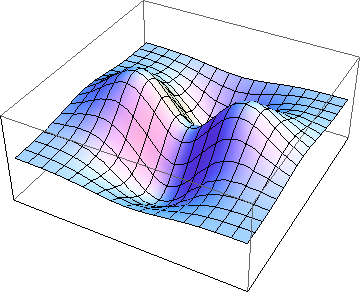
\includegraphics[width=0.8\textwidth]{images/partialdifferentiation.png}
			\end{center}
   	\end{columns}
}


\begin{frame}{Questions?}
	\begin{center}
		
\includegraphics[width=.7\textwidth]{images/fin.png}
	\end{center}
\end{frame}

\end{document}
